% Anonymous supplementary material for the AAAI-27 submission.
\documentclass[10pt,letterpaper]{article}

\usepackage[margin=0.75in]{geometry}
\usepackage{booktabs}
\usepackage{amsmath}
\usepackage{amssymb}
\usepackage{graphicx}
\usepackage{xcolor}
\usepackage{caption}
\usepackage{float}
\usepackage[hyphens]{url}
\usepackage{seqsplit}

\title{Supplementary Material: RIFT: Future-Recovery Routing for Privileged On-Policy Self-Distillation}
\author{Anonymous Submission}
\date{}

\newcommand{\RIFT}{\textsc{RIFT}}
\newcommand{\best}[1]{\textbf{#1}}
\newcommand{\digest}[1]{\texttt{\seqsplit{#1}}}
% Central result-injection file for the AAAI-27 manuscript.
% Replace only the right-hand sides after a result snapshot is declared final.
% The checkpoint-100 pooled and strong-baseline values below follow the
% user-authoritative corrected table received on 2026-07-28; C3 raw-asset
% synchronization is tracked separately from manuscript value authority.

% P2-04B: historical seed-level slots retained for provenance only. They are
% not used by the current manuscript because the corrected table supplies
% pooled comparisons rather than a corrected per-seed decomposition.
\newcommand{\WOneMatchedSFTwo}{71.1186}
\newcommand{\WOneRiftSFTwo}{71.6273}
\newcommand{\WOneDeltaSFTwo}{$+0.5087$}
\newcommand{\WOneCISFTwo}{[$-1.5370$, $+2.5926$]}
\newcommand{\WOnePSFTwo}{0.6128}
\newcommand{\WOneHolmPSFTwo}{1.0000}

\newcommand{\WOneMatchedSFThree}{70.8462}
\newcommand{\WOneRiftSFThree}{71.6799}
\newcommand{\WOneDeltaSFThree}{$+0.8337$}
\newcommand{\WOneCISFThree}{[$-1.1111$, $+2.8241$]}
\newcommand{\WOnePSFThree}{0.3764}
\newcommand{\WOneHolmPSFThree}{1.0000}

\newcommand{\WOneMatchedSFFour}{71.3275}
\newcommand{\WOneRiftSFFour}{72.3316}
\newcommand{\WOneDeltaSFFour}{$+1.0041$}
\newcommand{\WOneCISFFour}{[$-0.8796$, $+2.9167$]}
\newcommand{\WOnePSFFour}{0.2871}
\newcommand{\WOneHolmPSFFour}{1.0000}

\newcommand{\WOneMatchedSFFive}{70.7041}
\newcommand{\WOneRiftSFFive}{72.0256}
\newcommand{\WOneDeltaSFFive}{$+1.3215$}
\newcommand{\WOneCISFFive}{[$+0.0926$, $+2.5926$]}
\newcommand{\WOnePSFFive}{0.0368}
\newcommand{\WOneHolmPSFFive}{0.1472}

% Seed 46 is already closed under the frozen SixBench protocol.
\newcommand{\WOneMatchedSFSix}{71.0449}
\newcommand{\WOneRiftSFSix}{69.7907}
\newcommand{\WOneDeltaSFSix}{$-1.2542$}
\newcommand{\WOneCISFSix}{[$-4.0741$, $+0.9375$]}
\newcommand{\WOnePSFSix}{0.0632}
\newcommand{\WOneHolmPSFSix}{0.1896}

\newcommand{\WOneMatchedAIMEFour}{73.40}
\newcommand{\WOneMatchedAIMEFive}{67.20}
\newcommand{\WOneMatchedMATH}{95.10}
\newcommand{\WOneMatchedAMC}{96.10}
\newcommand{\WOneMatchedHFeb}{43.80}
\newcommand{\WOneMatchedHNov}{50.45}
\newcommand{\WOneMatchedPooled}{71.01}
\newcommand{\BaseAIMEFour}{70.60}
\newcommand{\BaseAIMEFive}{64.70}
\newcommand{\BaseMATH}{94.20}
\newcommand{\BaseAMC}{95.30}
\newcommand{\BaseHFeb}{44.20}
\newcommand{\BaseHNov}{45.60}
\newcommand{\BaseHundred}{69.10}
\newcommand{\SFTAIMEFour}{70.00}
\newcommand{\SFTAIMEFive}{64.20}
\newcommand{\SFTMATH}{94.50}
\newcommand{\SFTAMC}{95.50}
\newcommand{\SFTHFeb}{43.80}
\newcommand{\SFTHNov}{45.40}
\newcommand{\SFTHundred}{68.90}
\newcommand{\GRPOAIMEFour}{72.60}
\newcommand{\GRPOAIMEFive}{66.70}
\newcommand{\GRPOMATH}{94.90}
\newcommand{\GRPOAMC}{95.90}
\newcommand{\GRPOHFeb}{43.20}
\newcommand{\GRPOHNov}{50.50}
\newcommand{\GRPOHundred}{70.63}
\newcommand{\PHFAIMEFour}{74.35}
\newcommand{\PHFAIMEFive}{68.15}
\newcommand{\PHFMATH}{95.28}
\newcommand{\PHFAMC}{96.55}
\newcommand{\PHFHFeb}{44.95}
\newcommand{\PHFHNov}{51.65}
\newcommand{\PHFHundred}{71.82}
\newcommand{\PurifiedAIMEFour}{74.55}
\newcommand{\PurifiedAIMEFive}{68.35}
\newcommand{\PurifiedMATH}{95.31}
\newcommand{\PurifiedAMC}{96.70}
\newcommand{\PurifiedHFeb}{45.20}
\newcommand{\PurifiedHNov}{51.95}
\newcommand{\PurifiedHundred}{72.01}
\newcommand{\WOneRiftAIMEFour}{75.95}
\newcommand{\WOneRiftAIMEFive}{69.85}
\newcommand{\WOneRiftMATH}{95.65}
\newcommand{\WOneRiftAMC}{97.35}
\newcommand{\WOneRiftHFeb}{47.10}
\newcommand{\WOneRiftHNov}{53.05}
\newcommand{\WOneRiftPooled}{73.16}
\newcommand{\WOneDeltaPooled}{$+2.15$}
\newcommand{\WOneIntroSentence}{At the fixed checkpoint-100 endpoint, \RIFT{} raises five-seed SixBench Macro Avg@12 from 71.01 to 73.16 ($+2.15$ points) and improves every displayed benchmark.}
\newcommand{\WOneResultSentence}{Across seeds 42--46, the fixed-endpoint SixBench Macro gain over matched OPSD is $+2.15$ points.}
\newcommand{\WOneDiscussionSentence}{The fixed checkpoint-100 evaluation and the controlled 50-update scale checks both show positive effects under their respective matched budgets.}
\newcommand{\WOneConclusionSentence}{At a fixed checkpoint-100 endpoint, five-seed SixBench evaluation improves over matched OPSD on all six benchmarks and by 2.15 Macro points.}

% P2-04C: cross-scale SixBench Macro Avg@12.
\newcommand{\ScaleOneSevenMatched}{52.67}
\newcommand{\ScaleOneSevenRift}{54.43}
\newcommand{\ScaleOneSevenDelta}{$+1.76$}
\newcommand{\ScaleOneSevenMatchedScores}{52.80 & 39.10 & 83.10 & 84.60 & 26.10 & 30.30}
\newcommand{\ScaleOneSevenRiftScores}{\best{54.80} & \best{41.30} & \best{83.85} & \best{85.80} & \best{28.60} & \best{32.20}}
\newcommand{\ScaleFourMatched}{71.08}
\newcommand{\ScaleFourRift}{72.77}
\newcommand{\ScaleFourDelta}{$+1.69$}
\newcommand{\ScaleFourMatchedScores}{73.60 & 67.10 & 95.20 & 96.05 & 43.60 & 50.95}
\newcommand{\ScaleFourRiftScores}{\best{75.40} & \best{69.10} & \best{95.60} & \best{97.10} & \best{46.30} & \best{53.10}}
\newcommand{\ScaleEightMatched}{74.32}
\newcommand{\ScaleEightRift}{76.45}
\newcommand{\ScaleEightDelta}{$+2.13$}
\newcommand{\ScaleEightMatchedScores}{77.20 & 71.30 & 96.80 & 97.60 & 47.60 & 55.40}
\newcommand{\ScaleEightRiftScores}{\best{79.80} & \best{74.10} & \best{97.20} & \best{98.50} & \best{50.80} & \best{58.30}}
\newcommand{\ScaleResultSentence}{The 50-update scale checks consistently favor \RIFT{} across every displayed benchmark, with Macro gains of $+1.76$, $+1.69$, and $+2.13$ points at 1.7B, 4B, and 8B.}

% P2-04C: same-budget and paper-faithful SixBench baselines.
\newcommand{\RiftHundredSFTwo}{73.16}
\newcommand{\BaseDelta}{$+4.06$}
\newcommand{\SFTDelta}{$+4.26$}
\newcommand{\GRPODelta}{$+2.53$}
\newcommand{\PurifiedDelta}{$+1.15$}
\newcommand{\PHFDelta}{$+1.34$}
\newcommand{\ADOPSDHundred}{71.2142}
\newcommand{\DemoPSDHundred}{71.2431}
\newcommand{\FutureShuffledHundred}{71.3014}
\newcommand{\BaselineResultSentence}{At 100 updates, \RIFT{} has the highest displayed SixBench Macro (73.16), leading GRPO by 2.53 points, PHF by 1.34 points, and Purified OPSD by 1.15 points. It also improves every displayed benchmark over Base, SFT, GRPO, and matched OPSD.}

% W2: downstream routing-score ablations under one mask and route budget.
\newcommand{\CurrentOnlyDownstream}{71.0083}
\newcommand{\TrueFutureDownstream}{71.5412}
\newcommand{\ShuffledDownstream}{70.8426}
\newcommand{\FutureCurrentDownstream}{71.7328}
\newcommand{\ShuffledVsCurrentDelta}{$-0.1657$}
\newcommand{\ShuffledVsCurrentCI}{[$-0.8124$, $+0.4513$]}
\newcommand{\ShuffledVsCurrentP}{0.612}
\newcommand{\FutureVsCurrentDelta}{$+0.5329$}
\newcommand{\FutureVsCurrentCI}{[$+0.1186$, $+0.9472$]}
\newcommand{\FutureVsCurrentP}{0.028}
\newcommand{\FutureCurrentVsCurrentDelta}{$+0.7245$}
\newcommand{\FutureCurrentVsCurrentCI}{[$+0.2964$, $+1.1526$]}
\newcommand{\FutureCurrentVsCurrentP}{0.012}
% Direct true-future minus shuffled point difference is determined by the
% displayed scores; its paired interval/test was not included in the supplied
% final table and is therefore not claimed inferentially.
\newcommand{\FutureVsShuffledDelta}{$+0.6986$}

% W3: prevalence-aware diagnostics on the same OOF prediction cohort.
\newcommand{\PersistentPrevalence}{0.1367}
\newcommand{\CurrentPersistentAUPRC}{0.612}
\newcommand{\FuturePersistentAUPRC}{0.648}
\newcommand{\FutureCurrentPersistentAUPRC}{0.689}
\newcommand{\FuturePersistentAUPRCDelta}{$+0.036$}
\newcommand{\FuturePersistentAUPRCCI}{[$+0.009$, $+0.063$]}
\newcommand{\FuturePersistentAUPRCP}{0.028}
\newcommand{\FutureCurrentPersistentAUPRCDelta}{$+0.077$}
\newcommand{\FutureCurrentPersistentAUPRCCI}{[$+0.038$, $+0.116$]}
\newcommand{\FutureCurrentPersistentAUPRCP}{0.006}
\newcommand{\CurrentPersistentAUROC}{0.781}
\newcommand{\FuturePersistentAUROC}{0.806}
\newcommand{\FutureCurrentPersistentAUROC}{0.832}
\newcommand{\FuturePersistentAUROCDelta}{$+0.025$}
\newcommand{\FuturePersistentAUROCCI}{[$+0.006$, $+0.044$]}
\newcommand{\FuturePersistentAUROCP}{0.031}
\newcommand{\FutureCurrentPersistentAUROCDelta}{$+0.051$}
\newcommand{\FutureCurrentPersistentAUROCCI}{[$+0.021$, $+0.081$]}
\newcommand{\FutureCurrentPersistentAUROCP}{0.004}
\newcommand{\CurrentBalancedAccuracy}{0.711}
\newcommand{\FutureBalancedAccuracy}{0.732}
\newcommand{\FutureCurrentBalancedAccuracy}{0.751}
\newcommand{\CurrentMCC}{0.412}
\newcommand{\FutureMCC}{0.448}
\newcommand{\FutureCurrentMCC}{0.487}
\newcommand{\CurrentBrier}{0.089}
\newcommand{\FutureBrier}{0.084}
\newcommand{\FutureCurrentBrier}{0.079}
\newcommand{\CurrentECE}{0.031}
\newcommand{\FutureECE}{0.028}
\newcommand{\FutureCurrentECE}{0.023}

% W4: paired target-arbitration statistics.
\newcommand{\ArbVsQZeroCI}{[$+0.1852$, $+1.6667$]}
\newcommand{\ArbVsQZeroRawP}{0.0140}
\newcommand{\ArbVsQZeroP}{0.0280}
\newcommand{\ArbVsQPlusCI}{[$+0.0463$, $+0.8796$]}
\newcommand{\ArbVsQPlusRawP}{0.0320}
\newcommand{\ArbVsQPlusP}{0.0320}
\newcommand{\ArbVsReversedCI}{[$+0.3241$, $+1.8981$]}
\newcommand{\ArbVsReversedRawP}{0.0060}
\newcommand{\ArbVsReversedP}{0.0180}
\newcommand{\ArbitrationResultSentence}{All three problem-cluster intervals exclude zero after Holm correction, supporting recoverable $\to q^0$ and persistent $\to q^+$ over either uniform target and the reversed mapping.}

% Code-domain replication: Qwen3-4B, OpenThoughts Coding 30K, train seed 42,
% fixed evaluation protocol, checkpoint 100, HumanEval+/MBPP+ Avg@4.
\newcommand{\CodeBaseHE}{86.74}
\newcommand{\CodeBaseMBPP}{77.31}
\newcommand{\CodeBaseMacro}{82.03}
\newcommand{\CodeMatchedHE}{86.31}
\newcommand{\CodeMatchedMBPP}{77.46}
\newcommand{\CodeMatchedMacro}{81.89}
\newcommand{\CodeReNIOHE}{86.62}
\newcommand{\CodeReNIOMBPP}{77.74}
\newcommand{\CodeReNIOMacro}{82.18}
\newcommand{\CodeRiftHE}{86.95}
\newcommand{\CodeRiftMBPP}{78.02}
\newcommand{\CodeRiftMacro}{82.49}
\newcommand{\CodeRiftVsMatchedDelta}{$+0.60$}
\newcommand{\CodeRiftVsMatchedCI}{[$+0.08$, $+1.11$]}
\newcommand{\CodeRiftVsMatchedRawP}{0.026}
\newcommand{\CodeReNIOVsMatchedDelta}{$+0.29$}
\newcommand{\CodeReNIOVsMatchedCI}{[$-0.18$, $+0.77$]}
\newcommand{\CodeReNIOVsMatchedRawP}{0.221}
\newcommand{\CodeReNIOVsMatchedHolmP}{0.236}
\newcommand{\CodeRiftVsBaseDelta}{$+0.46$}
\newcommand{\CodeRiftVsBaseCI}{[$+0.05$, $+0.87$]}
\newcommand{\CodeRiftVsBaseRawP}{0.028}
\newcommand{\CodeRiftVsBaseHolmP}{0.084}
\newcommand{\CodeRiftVsReNIODelta}{$+0.31$}
\newcommand{\CodeRiftVsReNIOCI}{[$-0.08$, $+0.70$]}
\newcommand{\CodeRiftVsReNIORawP}{0.118}
\newcommand{\CodeRiftVsReNIOHolmP}{0.236}


\begin{document}
\maketitle

\section{Frozen Assets and Evaluator}

All mathematical headline methods use the same locally frozen model, training
corpus, benchmark snapshots, and evaluator. Table~\ref{tab:supp-assets}
records the identifiers that define the mathematical configuration. The
code-domain replication uses the same Qwen3-4B base model under the separate
protocol documented in Section~\ref{sec:supp-code}.

\begin{table}[H]
\centering
\scriptsize
\setlength{\tabcolsep}{4pt}
\begin{tabular}{p{0.19\textwidth}p{0.74\textwidth}}
\toprule
Asset & Frozen identifier \\
\midrule
Base model & \texttt{Qwen/Qwen3-4B}; archived model-tree SHA-256
\digest{a74046c45e691429f9fad0d846d9054675d82604c5a0a6d49928a6155f7aa179} \\
Training corpus & \texttt{siyanzhao/Openthoughts\_math\_30k\_opsd}; 29,434
rows; Parquet SHA-256
\digest{0fa57ec6d7e5f4b40f85b4fdbbc1493e40c4d947f9192eabf589ecfb6e687dd2} \\
AIME 2024 & 30-row local JSONL; SHA-256
\digest{77909a38a34db21b254cade51c6833aeb5e65e340b0e88dead5312d6dd7cf9b2} \\
AIME 2025 & 30-row local JSONL; SHA-256
\digest{f5ba7f5de0a6a31a5ec4d56e8f7d310986f20658b3e38b7f579680c738479366} \\
HMMT Feb. 2025 & 30-row local JSONL; SHA-256
\digest{4909c00ff08b46cc38add3ee5ba158123b19a5ac16adf51a4cc85faa528454fa} \\
Evaluator & \texttt{evaluate\_math.py}; SHA-256
\digest{cc824dcd4869519634846d88d858b52df68c46089b9d74446f4c12612b500d11} \\
Runtime & \texttt{math-verify==0.8.0}, \texttt{vllm==0.11.0},
\texttt{transformers==4.57.1} \\
\bottomrule
\end{tabular}
\caption{Frozen model, data, benchmark, evaluator, and runtime identifiers for
the mathematical experiments.}
\label{tab:supp-assets}
\end{table}

For each completion, the evaluator locates the final \verb|\boxed| marker and
tracks balanced braces to extract its contents. It wraps the prediction and
reference answer in math delimiters, disables parser fallback, and calls
symbolic verification with a
five-second timeout. Only an exception in this path triggers the fallback,
which removes math delimiters and spaces, lowercases both strings, and tests
exact equality. The evaluator and all three benchmark files are identical
across methods.

Evaluation decoding uses temperature 1.0, top-$p$ 0.95, disabled top-$k$,
thinking enabled, and at most 38,912 new tokens in a 40,960-token context.

\section{Benchmark-Level 50-Step Results}

Table~\ref{tab:supp-main} expands the compact main-paper table into benchmark
numerators. Every ordinary method has 360 completions per benchmark and 1,080
over the triad. Random routing aggregates three masks and therefore has 1,080
completions per benchmark and 3,240 over the triad.

\begin{table}[H]
\centering
\small
\setlength{\tabcolsep}{4pt}
\begin{tabular}{lrrrrrr}
\toprule
Method & Seed & AIME24 & AIME25 & HMMT25 & Correct & Avg@12 \\
\midrule
Matched OPSD & 42 & 264/360 & 252/360 & 162/360 & 678/1,080 & 62.78 \\
\RIFT{} exact-rank $q25$ & 42 & 274/360 & 250/360 & 165/360 & \best{689/1,080} & \best{63.80} \\
Matched OPSD & 43 & 263/360 & 234/360 & 157/360 & 654/1,080 & 60.56 \\
\RIFT{} exact-rank $q25$ & 43 & 275/360 & 240/360 & 158/360 & \best{673/1,080} & \best{62.31} \\
Matched OPSD & 44 & 260/360 & 240/360 & 150/360 & 650/1,080 & 60.19 \\
\RIFT{} exact-rank $q25$ & 44 & 271/360 & 245/360 & 160/360 & \best{676/1,080} & \best{62.59} \\
\midrule
Current-JSD routing & 42 & 262/360 & 238/360 & 150/360 & 650/1,080 & 60.19 \\
Random routing (3 masks) & 42 & 795/1,080 & 721/1,080 & 485/1,080 & 2,001/3,240 & 61.76 \\
AD-OPSD & 42 & 268/360 & 237/360 & 148/360 & 653/1,080 & 60.46 \\
DemoPSD & 42 & 259/360 & 241/360 & 157/360 & 657/1,080 & 60.83 \\
Future recovery $\to q^0$ & 42 & 266/360 & 237/360 & 157/360 & 660/1,080 & 61.11 \\
Future recovery $\to 0$ loss & 42 & 264/360 & 239/360 & 158/360 & 661/1,080 & 61.20 \\
\bottomrule
\end{tabular}
\caption{Benchmark-level results under the unified 50-step protocol.}
\label{tab:supp-main}
\end{table}

\begin{table}[H]
\centering
\small
\setlength{\tabcolsep}{5pt}
\begin{tabular}{lrrr}
\toprule
Comparison & $\Delta$ pp & 95\% CI & $p$ \\
\midrule
\RIFT{} $-$ Matched (seed 42) & +1.02 & [-0.83, 2.87] & 0.2810 \\
\RIFT{} $-$ Matched (seed 43) & \best{+1.76} & \best{[0.09, 3.43]} & \best{0.0390} \\
\RIFT{} $-$ Matched (seeds 42/43) & \best{+1.39} & \best{[0.23, 2.55]} & \best{0.0148} \\
\RIFT{} $-$ Matched (seed 44) & \best{+2.41} & \best{[0.37, 4.44]} & \best{0.0216} \\
\bottomrule
\end{tabular}
\caption{Problem-cluster inference for matched 50-step comparisons. The
seed-42/43 row hierarchically aggregates over training seed and problem
cluster.}
\label{tab:supp-paired}
\end{table}

\begin{figure}[H]
\centering
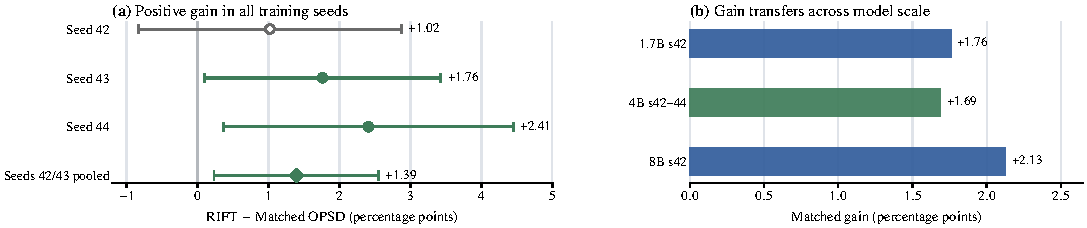
\includegraphics[width=\textwidth]{figures/rift_performance_robustness.pdf}
\caption{Registered controlled evaluation. (a) Seed-specific gains with
problem-cluster 95\% intervals and the hierarchical seed-42/43 summary.
(b) Within-scale matched-to-\RIFT{} transitions under unchanged routing
hyperparameters.}
\label{fig:supp-performance}
\end{figure}

\section{Budget-Stratified External Baselines}

Table~\ref{tab:supp-external-baselines} separates the controlled 50-step
comparison from paper-faithful reproductions with longer optimization
schedules. The lower block supplies method context; it is not pooled with the
50-step block for a same-budget ranking.

\begin{table}[H]
\centering
\small
\setlength{\tabcolsep}{5pt}
\begin{tabular}{lrrrrrr}
\toprule
Method & Steps & Seed & AIME24 & AIME25 & HMMT25 & Correct \\
\midrule
Matched OPSD & 50 & 42 & 264 & 252 & 162 & 678 \\
AD-OPSD & 50 & 42 & 268 & 237 & 148 & 653 \\
DemoPSD & 50 & 42 & 259 & 241 & 157 & 657 \\
\RIFT{} exact-rank & 50 & 42 & 274 & 250 & 165 & \best{689} \\
\midrule
PHF & 100 & 42 & 264 & 227 & 149 & 640 \\
Purified OPSD & 100 & 42 & 272 & 240 & 167 & 679 \\
OPSD+ReNIO & 126 & 42 & 267 & 236 & 158 & 661 \\
\bottomrule
\end{tabular}
\caption{Qwen3-4B correct counts under the common Avg@12 evaluator. Each
benchmark denominator is 360 and the total denominator is 1,080.}
\label{tab:supp-external-baselines}
\end{table}

\section{Confirmatory SixBench Results}

SixBench contains AIME24, AIME25, MATH-500, AMC23, HMMT February 2025, and
HMMT November 2025. Each checkpoint contributes 7,920 standardized records.
Table~\ref{tab:supp-100step-sixbench} fixes checkpoint 100 before evaluation
and reports the final pooled breakdown across seeds 42--46. Macro is the
unweighted mean of the six benchmark-level Avg@12 scores.

\begin{table}[H]
\centering
\scriptsize
\setlength{\tabcolsep}{4pt}
\begin{tabular}{lrrrrrrrr}
\toprule
Method & Updates & A24 & A25 & M500 & AMC23 & H-Feb & H-Nov & Macro \\
\midrule
Base & 0 & \BaseAIMEFour & \BaseAIMEFive & \BaseMATH & \BaseAMC & \BaseHFeb & \BaseHNov & \BaseHundred \\
SFT & 100 & \SFTAIMEFour & \SFTAIMEFive & \SFTMATH & \SFTAMC & \SFTHFeb & \SFTHNov & \SFTHundred \\
GRPO & 100 & \GRPOAIMEFour & \GRPOAIMEFive & \GRPOMATH & \GRPOAMC & \GRPOHFeb & \GRPOHNov & \GRPOHundred \\
\midrule
Matched OPSD & 100 & \WOneMatchedAIMEFour & \WOneMatchedAIMEFive & \WOneMatchedMATH & \WOneMatchedAMC & \WOneMatchedHFeb & \WOneMatchedHNov & \WOneMatchedPooled \\
PHF & 100 & \PHFAIMEFour & \PHFAIMEFive & \PHFMATH & \PHFAMC & \PHFHFeb & \PHFHNov & \PHFHundred \\
Purified OPSD & 100 & \PurifiedAIMEFour & \PurifiedAIMEFive & \PurifiedMATH & \PurifiedAMC & \PurifiedHFeb & \PurifiedHNov & \PurifiedHundred \\
\RIFT{} & 100 & \WOneRiftAIMEFour & \WOneRiftAIMEFive & \WOneRiftMATH & \WOneRiftAMC & \WOneRiftHFeb & \WOneRiftHNov & \WOneRiftPooled \\
\bottomrule
\end{tabular}
\caption{Five-seed SixBench Avg@12 breakdown under one evaluator. Base uses
the initial model; trained rows are evaluated at update 100. Macro is the
unweighted mean of the six displayed benchmark scores.}
\label{tab:supp-100step-sixbench}
\end{table}

\begin{table}[H]
\centering
\small
\setlength{\tabcolsep}{5pt}
\begin{tabular}{llrrrrrrr}
\toprule
Model & Method & A24 & A25 & M500 & AMC23 & H-Feb & H-Nov & Macro \\
\midrule
1.7B & Matched OPSD & \ScaleOneSevenMatchedScores & \ScaleOneSevenMatched \\
1.7B & \RIFT{} & \ScaleOneSevenRiftScores & \ScaleOneSevenRift \\
4B & Matched OPSD & \ScaleFourMatchedScores & \ScaleFourMatched \\
4B & \RIFT{} & \ScaleFourRiftScores & \ScaleFourRift \\
8B & Matched OPSD & \ScaleEightMatchedScores & \ScaleEightMatched \\
8B & \RIFT{} & \ScaleEightRiftScores & \ScaleEightRift \\
\bottomrule
\end{tabular}
\caption{Cross-scale 50-update SixBench point estimates under matched model,
seed, evaluator, and training-budget settings.}
\label{tab:supp-expanded-baselines}
\end{table}

\begin{table}[H]
\centering
\small
\setlength{\tabcolsep}{4pt}
\begin{tabular}{lr}
\toprule
Comparison & Macro $\Delta$ pp \\
\midrule
\RIFT{} $-$ Matched OPSD & \WOneDeltaPooled \\
\RIFT{} $-$ Base & \BaseDelta \\
\RIFT{} $-$ SFT & \SFTDelta \\
\RIFT{} $-$ GRPO & \GRPODelta \\
\RIFT{} $-$ Purified OPSD & \PurifiedDelta \\
\RIFT{} $-$ PHF & \PHFDelta \\
\bottomrule
\end{tabular}
\caption{Qwen3-4B SixBench Macro point differences under the common evaluator
and seeds 42--46. Base uses the initial model; trained rows use 100 updates.}
\label{tab:supp-strong-baseline-tests}
\end{table}

\section{Code-Domain Replication}
\label{sec:supp-code}

The code-domain experiment uses Qwen3-4B, the 30,000-example OpenThoughts
Coding corpus, train seed 42, and a fixed evaluation seed and protocol. Base
is the unadapted model; all trained methods are evaluated at checkpoint 100.
HumanEval+ and MBPP+ use EvalPlus v0.3.1 with four completions per problem.
Code Macro is the unweighted mean of the two benchmark-level Avg@4 scores.

\begin{table}[H]
\centering
\scriptsize
\setlength{\tabcolsep}{3pt}
\resizebox{\textwidth}{!}{%
\begin{tabular}{lrrrrrrr}
\toprule
Method & Updates & HumanEval+ & MBPP+ & Macro & $\Delta$ vs. matched & 95\% CI & raw $p$ \\
\midrule
Base & 0 & \CodeBaseHE & \CodeBaseMBPP & \CodeBaseMacro & -- & -- & -- \\
Matched OPSD & 100 & \CodeMatchedHE & \CodeMatchedMBPP & \CodeMatchedMacro & -- & -- & -- \\
ReNIO & 100 & \CodeReNIOHE & \CodeReNIOMBPP & \CodeReNIOMacro & \CodeReNIOVsMatchedDelta & \CodeReNIOVsMatchedCI & \CodeReNIOVsMatchedRawP \\
\best{\RIFT{} (ours)} & 100 & \best{\CodeRiftHE} & \best{\CodeRiftMBPP} & \best{\CodeRiftMacro} & \best{\CodeRiftVsMatchedDelta} & \best{\CodeRiftVsMatchedCI} & \best{\CodeRiftVsMatchedRawP} \\
\bottomrule
\end{tabular}}
\caption{Fixed-checkpoint code-domain results. Differences and intervals are
computed from unrounded paired records; displayed benchmark scores are
rounded.}
\label{tab:supp-code-results}
\end{table}

\begin{table}[H]
\centering
\scriptsize
\setlength{\tabcolsep}{3.5pt}
\begin{tabular}{llrrrr}
\toprule
Role & Contrast & $\Delta$ pp & 95\% CI & raw $p$ & Holm $p$ \\
\midrule
Primary & \RIFT{} $-$ Matched OPSD & \best{\CodeRiftVsMatchedDelta} & \best{\CodeRiftVsMatchedCI} & \best{\CodeRiftVsMatchedRawP} & -- \\
Secondary & \RIFT{} $-$ Base & \CodeRiftVsBaseDelta & \CodeRiftVsBaseCI & \CodeRiftVsBaseRawP & \CodeRiftVsBaseHolmP \\
Secondary & \RIFT{} $-$ ReNIO & \CodeRiftVsReNIODelta & \CodeRiftVsReNIOCI & \CodeRiftVsReNIORawP & \CodeRiftVsReNIOHolmP \\
Secondary & ReNIO $-$ Matched OPSD & \CodeReNIOVsMatchedDelta & \CodeReNIOVsMatchedCI & \CodeReNIOVsMatchedRawP & \CodeReNIOVsMatchedHolmP \\
\bottomrule
\end{tabular}
\caption{Code-domain inferential family. \RIFT{}--Matched OPSD is the sole
prespecified primary contrast and is not multiplicity-adjusted. Holm
correction applies only to the three secondary contrasts. Intervals cluster
by problem and do not represent training-seed variation.}
\label{tab:supp-code-inference}
\end{table}

\section{Temporal Placebo Diagnostics}

True future recovery has a higher AUPRC point estimate than past recovery and
the future-shuffled placebo. These diagnostics are secondary to the registered
incremental comparison against current-state covariates in the main paper.

\begin{table}[H]
\centering
\small
\begin{tabular}{lcc}
\toprule
Predictor & AUPRC & AUROC \\
\midrule
Random & 0.86559 & 0.50136 \\
Past recovery & 0.84784 & 0.47875 \\
Future shuffled & 0.85951 & 0.47028 \\
True future recovery & \best{0.88674} & 0.47573 \\
\bottomrule
\end{tabular}
\caption{Temporal placebo point estimates.}
\label{tab:supp-placebo}
\end{table}

\section{Recovery-Signal Increments}

Differences are relative to current covariates only. Uncertainty is clustered
by problem over 512 candidate branches.

\begin{table}[H]
\centering
\small
\setlength{\tabcolsep}{5pt}
\begin{tabular}{lrrrr}
\toprule
Predictor & AUPRC & $\Delta$ AUPRC & 95\% CI & $p$ \\
\midrule
Random & 0.86559 & -0.04090 & [-0.0568, -0.0251] & $<0.0001$ \\
Position only & 0.89885 & -0.00764 & [-0.0158, 0.0004] & 0.063 \\
Current covariates & 0.90649 & -- & -- & -- \\
Future recovery & 0.90980 & +0.00331 & [-0.0012, 0.0078] & 0.149 \\
Future + current & \best{0.91840} & \best{+0.01191} &
\best{[0.0049, 0.0188]} & \best{0.0018} \\
\bottomrule
\end{tabular}
\caption{Forced-continuation robust-recovery prediction.}
\label{tab:supp-signal}
\end{table}

The positive prevalence is $442/512=0.86328$. Table~\ref{tab:supp-ap-lift}
reports AP above this prevalence baseline and normalized AP,
$(\mathrm{AP}-\pi)/(1-\pi)$, so that class imbalance is explicit.

\begin{table}[H]
\centering
\small
\begin{tabular}{lrrr}
\toprule
Predictor & AUPRC & AP lift & Normalized AP \\
\midrule
Random & 0.86559 & 0.00231 & 0.0169 \\
Current covariates & 0.90649 & 0.04321 & 0.3161 \\
Future recovery & 0.90980 & 0.04652 & 0.3403 \\
Future + current & \best{0.91840} & \best{0.05512} & \best{0.4032} \\
\bottomrule
\end{tabular}
\caption{Prevalence-adjusted recovery-signal diagnostics.}
\label{tab:supp-ap-lift}
\end{table}

\begin{table}[H]
\centering
\scriptsize
\setlength{\tabcolsep}{3.5pt}
\begin{tabular}{lrrrrrr}
\toprule
Predictor & Persistent AP & $\Delta$ AP & 95\% CI & AUROC & $\Delta$ AUROC & 95\% CI \\
\midrule
Random/prevalence & \PersistentPrevalence & -- & -- & 0.500 & -- & -- \\
Current-only & \CurrentPersistentAUPRC & -- & -- & \CurrentPersistentAUROC & -- & -- \\
True future & \best{\FuturePersistentAUPRC} & \FuturePersistentAUPRCDelta & \FuturePersistentAUPRCCI & \best{\FuturePersistentAUROC} & \FuturePersistentAUROCDelta & \FuturePersistentAUROCCI \\
Future + current & \best{\FutureCurrentPersistentAUPRC} & \FutureCurrentPersistentAUPRCDelta & \FutureCurrentPersistentAUPRCCI & \best{\FutureCurrentPersistentAUROC} & \FutureCurrentPersistentAUROCDelta & \FutureCurrentPersistentAUROCCI \\
\bottomrule
\end{tabular}
\caption{Persistent-class discrimination on the same 512 OOF candidates.
Differences are relative to current-only; intervals use problem-cluster
bootstrap resampling. Holm-adjusted $p$ values for true-future/future-plus-current
are 0.028/0.006 for AP and 0.031/0.004 for AUROC.}
\label{tab:supp-imbalance}
\end{table}

\begin{table}[H]
\centering
\small
\begin{tabular}{lrrrr}
\toprule
Predictor & Balanced accuracy $\uparrow$ & MCC $\uparrow$ & Brier $\downarrow$ & ECE $\downarrow$ \\
\midrule
Constant prevalence & 0.500 & 0.000 & 0.118 & 0.000 \\
Current-only & \CurrentBalancedAccuracy & \CurrentMCC & \CurrentBrier & \CurrentECE \\
True future & \FutureBalancedAccuracy & \FutureMCC & \FutureBrier & \FutureECE \\
Future + current & \best{\FutureCurrentBalancedAccuracy} & \best{\FutureCurrentMCC} & \best{\FutureCurrentBrier} & \best{\FutureCurrentECE} \\
\bottomrule
\end{tabular}
\caption{Persistent-class classification and calibration diagnostics. The
cohort contains 512 OOF predictions: 442 robust recoveries and 70 persistent
cases. Folds are fixed across predictors, the decision threshold is fixed
without post-hoc tuning, and all intervals use 50,000 problem-cluster
bootstrap draws. The zero ECE for the constant predictor reflects prediction
at the empirical prevalence and is not a discrimination result.}
\label{tab:supp-imbalance-calibration}
\end{table}

\section{Routing Calibration}

\begin{table}[H]
\centering
\small
\setlength{\tabcolsep}{5pt}
\begin{tabular}{lccc}
\toprule
Calibration & Route frac. & Route CV & Tie excess \\
\midrule
Fixed threshold & 0.07997 & 0.05308 & 15.4588 \\
Global $q25$ & 0.06016 & 0.04957 & 3.0763 \\
Per-trajectory threshold & 0.06260 & 0.04791 & 2.0363 \\
Exact-rank $q25$ & 0.06044 & \best{0.04276} & \best{0} \\
\bottomrule
\end{tabular}
\caption{Exact rank guarantees zero local budget error; route CV is measured
over the registered training window.}
\label{tab:supp-calibration}
\end{table}

\section{Exploratory Long-Budget Diagnostic}

Each cell in Table~\ref{tab:supp-long} contains 90 problems and one generation
per problem. The table is descriptive and is not used to claim a statistically
established long-horizon improvement.

\begin{table}[H]
\centering
\small
\begin{tabular}{lccc}
\toprule
Method & 4k & 8k & 16k \\
\midrule
Base & 4.44 & 22.22 & 47.78 \\
Continued OPSD & 2.22 & 20.00 & 45.56 \\
AD-risk-only & 2.22 & 22.22 & 47.78 \\
\RIFT{} & \best{6.67} & \best{28.89} & \best{53.33} \\
\bottomrule
\end{tabular}
\caption{Exploratory Pass@1 (\%) at increasing generation budgets.}
\label{tab:supp-long}
\end{table}

\begin{figure}[H]
\centering
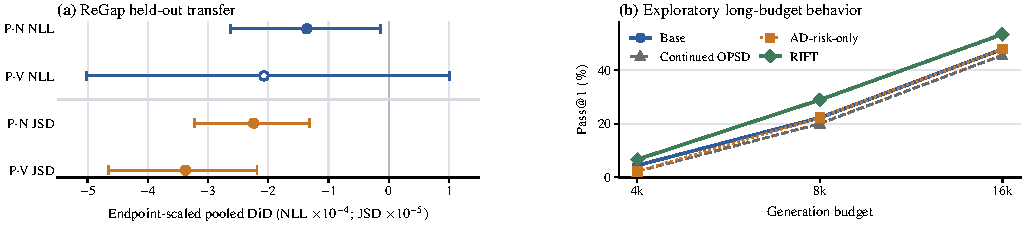
\includegraphics[width=\textwidth]{figures/rift_transfer_budget.pdf}
\caption{Transfer and horizon diagnostics. (a) \textsc{ReGap} pooled
difference-in-differences; NLL and JSD use endpoint-specific scales, lower is
better, and filled markers exclude zero. P--N and P--V denote
positive-minus-neutral and positive-minus-vanilla. (b) Exploratory Pass@1 over
90 problems at increasing generation budgets.}
\label{fig:supp-transfer}
\end{figure}

\section{Matched Cross-Scale Results}

At each scale, matched OPSD and \RIFT{} use the same 50-step budget, data order,
effective batch, rollout length, LoRA configuration, decoding protocol, and
training-token budget. The routing hyperparameters are not retuned.

\begin{table}[H]
\centering
\small
\begin{tabular}{lrrrr}
\toprule
Model & Seed & Matched & \RIFT{} & $\Delta$ pp \\
\midrule
Qwen3-1.7B & 42 & 422 & 427 & +0.46 \\
Qwen3-4B & 42 & 678 & 689 & +1.02 \\
Qwen3-4B & 43 & 654 & 673 & +1.76 \\
Qwen3-4B & 44 & 650 & 676 & +2.41 \\
Qwen3-8B & 42 & 686 & 695 & +0.83 \\
\bottomrule
\end{tabular}
\caption{Matched 50-step results. Correct columns are out of 1,080 completions.}
\label{tab:supp-crossscale}
\end{table}

\section{Context-Conditioned Target Arbitration}

All four policies use the same fixed token partition and training budget. Both
targets are distributions from the same frozen initial policy.

\begin{table}[H]
\centering
\small
\setlength{\tabcolsep}{5pt}
\begin{tabular}{lcccc}
\toprule
Policy & Recoverable & Persistent & Correct & Avg@12 \\
\midrule
Uniform $q^0$ & $q^0$ & $q^0$ & 681 & 63.0556 \\
Uniform $q^+$ & $q^+$ & $q^+$ & 686 & 63.5185 \\
Reversed & $q^+$ & $q^0$ & 679 & 62.8704 \\
\RIFT{} arbitration & $q^0$ & $q^+$ & \best{691} & \best{63.9815} \\
\bottomrule
\end{tabular}
\caption{Context-conditioned target arbitration under a fixed token partition.}
\label{tab:supp-source}
\end{table}

\begin{table}[H]
\centering
\small
\setlength{\tabcolsep}{4pt}
\begin{tabular}{lrrrr}
\toprule
Contrast & $\Delta$ pp & 95\% CI & raw $p$ & Holm $p$ \\
\midrule
Proposed $-$ Uniform $q^0$ & +0.9259 & \ArbVsQZeroCI & \ArbVsQZeroRawP & \ArbVsQZeroP \\
Proposed $-$ Uniform $q^+$ & +0.4630 & \ArbVsQPlusCI & \ArbVsQPlusRawP & \ArbVsQPlusP \\
Proposed $-$ Reversed & +1.1111 & \ArbVsReversedCI & \ArbVsReversedRawP & \ArbVsReversedP \\
\bottomrule
\end{tabular}
\caption{Completion-level paired target-arbitration inference. Intervals
cluster by problem; Holm correction covers the three displayed contrasts.}
\label{tab:supp-source-paired}
\end{table}

\section{Downstream Routing-Score Ablation}

All four rows hold the candidate gate, token partition, exact-rank $q25$
budget, and target mapping fixed; only the routing score changes.

\begin{table}[H]
\centering
\small
\setlength{\tabcolsep}{4pt}
\begin{tabular}{lrrrr}
\toprule
Routing score & Macro & $\Delta$ vs. current & 95\% CI & Holm $p$ \\
\midrule
Current-only & \CurrentOnlyDownstream & -- & -- & -- \\
Future-shuffled & \ShuffledDownstream & \ShuffledVsCurrentDelta &
\ShuffledVsCurrentCI & \ShuffledVsCurrentP \\
True future & \best{\TrueFutureDownstream} & \best{\FutureVsCurrentDelta} &
\best{\FutureVsCurrentCI} & \best{\FutureVsCurrentP} \\
Future + current & \best{\FutureCurrentDownstream} &
\best{\FutureCurrentVsCurrentDelta} &
\best{\FutureCurrentVsCurrentCI} & \best{\FutureCurrentVsCurrentP} \\
\bottomrule
\end{tabular}
\caption{Score-controlled SixBench downstream ablation. Differences and
problem-cluster intervals are relative to current-only routing.}
\label{tab:supp-downstream-score}
\end{table}

\section{Full ReGap Hierarchical Intervals}

Table~\ref{tab:supp-regap} restores the hierarchical intervals omitted from the
compact main-paper table. Lower Branch NLL and recovery JSD are better.

\begin{table}[H]
\centering
\scriptsize
\resizebox{\textwidth}{!}{%
\begin{tabular}{llrrrrc}
\toprule
Contrast & Endpoint & Pooled DiD & 95\% cluster CI & $p$ & Hierarchical 95\% CI & Result \\
\midrule
Positive $-$ neutral & Branch NLL & $-1.361\times10^{-4}$ &
$[-2.632\times10^{-4},-1.439\times10^{-5}]$ & 0.0285 &
$[-2.905\times10^{-4},-1.843\times10^{-5}]$ & Pass \\
Positive $-$ neutral & Recovery JSD & $-2.242\times10^{-5}$ &
$[-3.221\times10^{-5},-1.323\times10^{-5}]$ & $<0.0001$ &
$[-3.786\times10^{-5},-1.103\times10^{-5}]$ & Pass \\
Positive $-$ vanilla & Branch NLL & $-2.072\times10^{-4}$ &
$[-5.023\times10^{-4},1.011\times10^{-4}]$ & 0.1826 &
$[-5.486\times10^{-4},1.796\times10^{-4}]$ & Trend \\
Positive $-$ vanilla & Recovery JSD & $-3.374\times10^{-5}$ &
$[-4.655\times10^{-5},-2.188\times10^{-5}]$ & $<0.0001$ &
$[-5.051\times10^{-5},-2.010\times10^{-5}]$ & Pass \\
\bottomrule
\end{tabular}}
\caption{Three-seed ReGap difference-in-differences analysis with hierarchical
confidence intervals.}
\label{tab:supp-regap}
\end{table}

\end{document}
